\documentclass[11pt,a4]{article}
\usepackage[cm]{fullpage}
\usepackage{graphicx}
\usepackage{subfigure}
\usepackage{epsfig}
\usepackage{epstopdf}
\begin{document}

\begin{figure}[h]
\centering
    \includegraphics[width=0.49\textwidth]{YY1}
    \includegraphics[width=0.49\textwidth]{SP2}
    \includegraphics[width=0.49\textwidth]{REST}
    \includegraphics[width=0.49\textwidth]{ARID3A}
\caption{ROC curve created when applying the methods to data from the cell line HepG2. All HMM Models were trained with data from H1-hESC and K562 cell lines.}
\label{fig:roc.HepG2.1}
\end{figure}

\begin{figure}[h]
\centering
    \includegraphics[width=0.49\textwidth]{BRCA1}
    \includegraphics[width=0.49\textwidth]{RAD21}
    \includegraphics[width=0.49\textwidth]{ATF3}
    \includegraphics[width=0.49\textwidth]{NRF1}
\caption{ROC curve created when applying the methods to data from the cell line HepG2. All HMM Models were trained with data from H1-hESC and K562 cell lines.}
\label{fig:roc.HepG2.2}
\end{figure}

\begin{figure}[h]
\centering
    \includegraphics[width=0.49\textwidth]{USF2}
    \includegraphics[width=0.49\textwidth]{JUND}
    \includegraphics[width=0.49\textwidth]{ELF1}
    \includegraphics[width=0.49\textwidth]{MAFK}
\caption{ROC curve created when applying the methods to data from the cell line HepG2. All HMM Models were trained with data from H1-hESC and K562 cell lines.}
\label{fig:roc.HepG2.3}
\end{figure}

\begin{figure}[h]
\centering
    \includegraphics[width=0.49\textwidth]{MYC}
    \includegraphics[width=0.49\textwidth]{SRF}
    \includegraphics[width=0.49\textwidth]{JUN}
    \includegraphics[width=0.49\textwidth]{TBP}
\caption{ROC curve created when applying the methods to data from the cell line HepG2. All HMM Models were trained with data from H1-hESC and K562 cell lines.}
\label{fig:roc.HepG2.4}
\end{figure}

\begin{figure}[h]
\centering
    \includegraphics[width=0.49\textwidth]{P300}
    \includegraphics[width=0.49\textwidth]{BHLHE40}
    \includegraphics[width=0.49\textwidth]{USF1}
    \includegraphics[width=0.49\textwidth]{RXRA}
\caption{ROC curve created when applying the methods to data from the cell line HepG2. All HMM Models were trained with data from H1-hESC and K562 cell lines.}
\label{fig:roc.HepG2.5}
\end{figure}

\begin{figure}[h]
\centering
    \includegraphics[width=0.49\textwidth]{MAFF}
    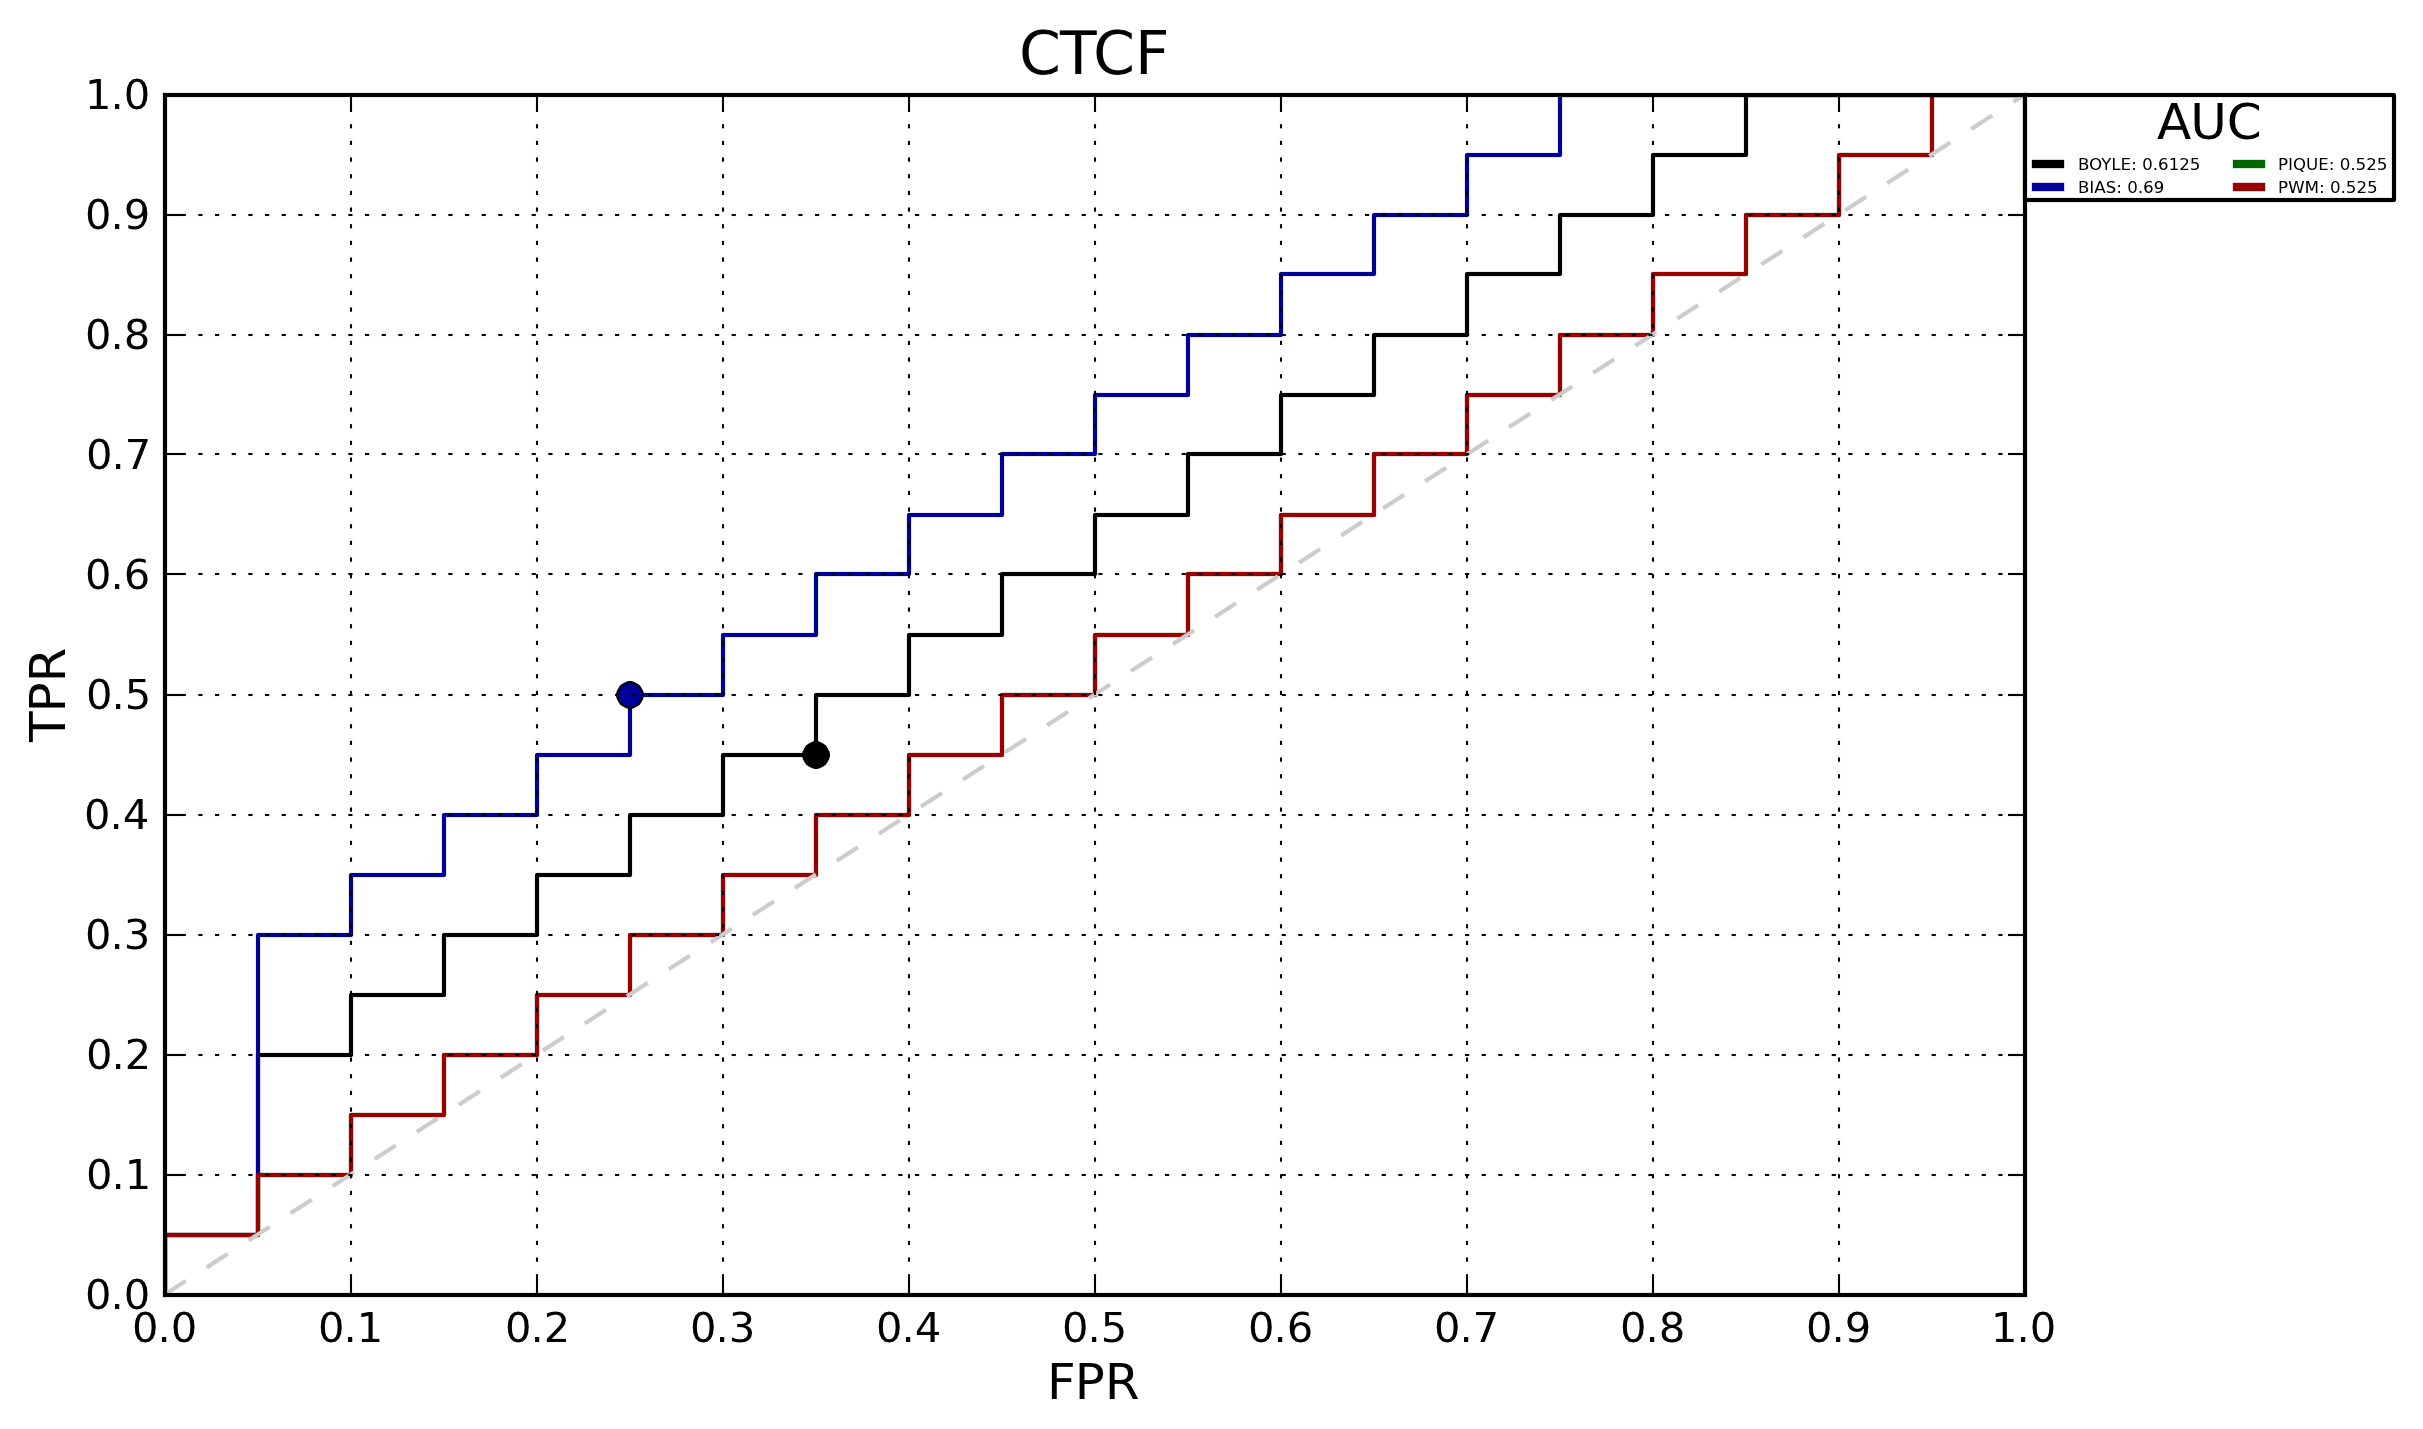
\includegraphics[width=0.49\textwidth]{CTCF}
    \includegraphics[width=0.49\textwidth]{MAX}
    \includegraphics[width=0.49\textwidth]{SP1}
\caption{ROC curve created when applying the methods to data from the cell line HepG2. All HMM Models were trained with data from H1-hESC and K562 cell lines.}
\label{fig:roc.HepG2.6}
\end{figure}

\begin{figure}[h]
\centering
    \includegraphics[width=0.49\textwidth]{CEBPB}
    \includegraphics[width=0.49\textwidth]{GABP}
\caption{ROC curve created when applying the methods to data from the cell line HepG2. All HMM Models were trained with data from H1-hESC and K562 cell lines.}
\label{fig:roc.HepG2.7}
\end{figure}

\end{document}